
	% perl -p -e 's/RU-/"RU-".++$i/ge' _REQS.tex > REQS.tex

	\req{ RU-1 }{Basic Functionality}{}{}
	{ The FirmWare has to access available hardware, to generate two-channel signals in ramp-, constant or arbitrary form, with 
	\begin{itemize} \setlength\itemsep{1px}
	\item sample-rates ( $\ne$ signal-frequency) up to 250kSPS
	\item a resolution of 16bit
	\item resulting in $\pm$10 volts of output voltage
	\end{itemize}
	
	}
	{}{}{}{General}
	\begin{center}
	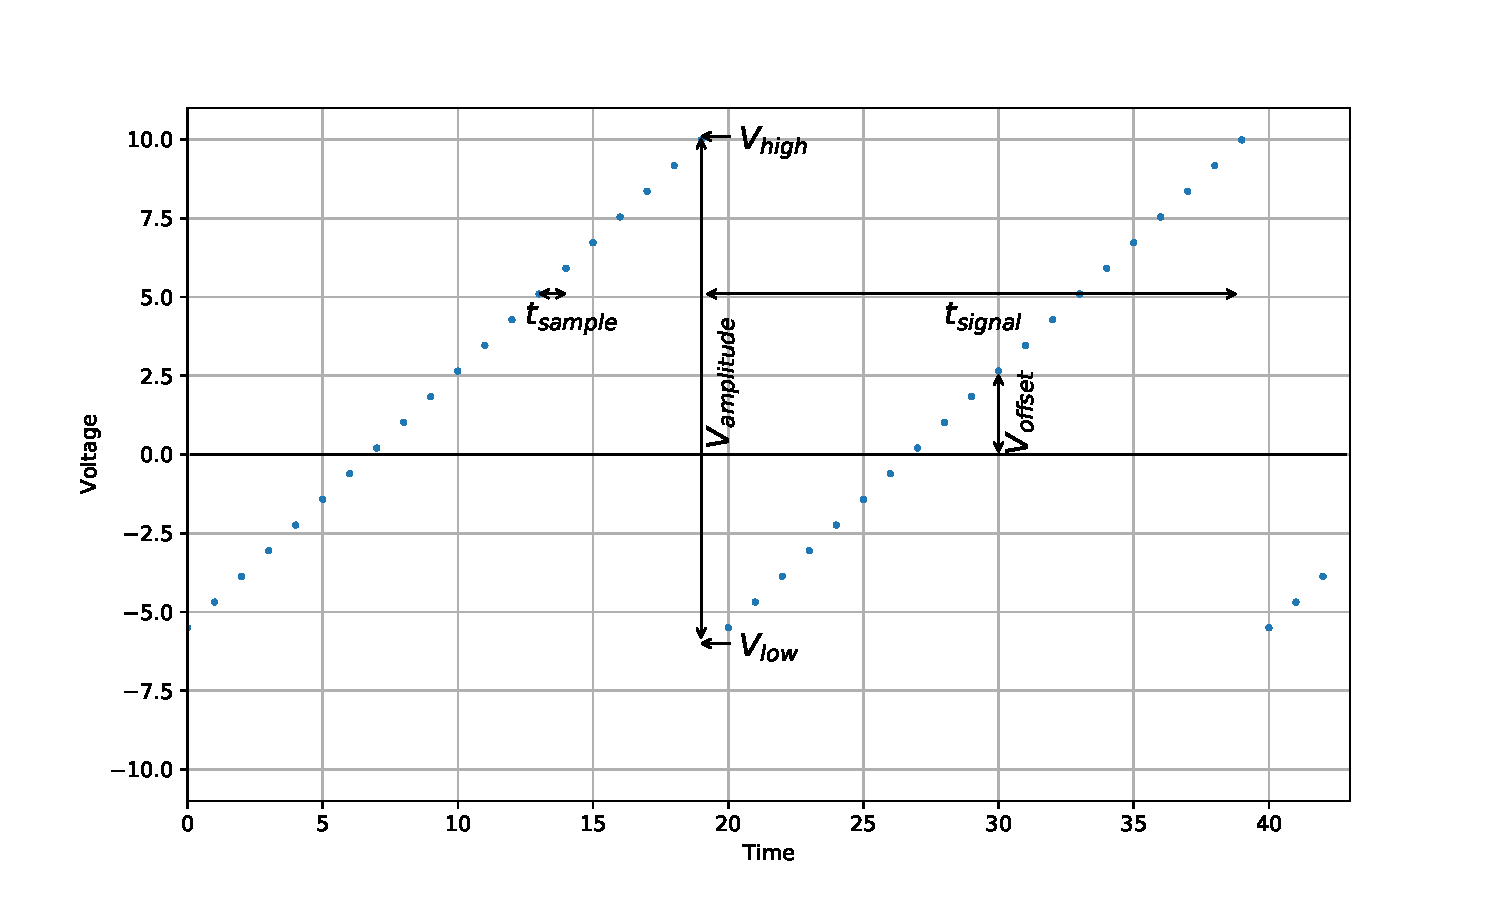
\includegraphics[width=0.99\textwidth, trim = {0 1.6cm 0 1.5cm}, clip]{src/_rampProperties.pdf}
	\end{center}
	\begin{align*}
	t_{sample} &\textrm{ ... sampling-time or -period, alias: trigger-rate } \\
	t_{signal} &\textrm{ ... signal-time or -period } \\
	f_{sample} &\textrm{ ... sampling-frequency or -rate } \\
	f_{signal} &\textrm{ ... signal-frequency or -rate } \\
	N &\textrm{ ... sample-count, length of the signal-vector } \\
	f_{sample} & = \frac{1}{t_{sample}} = N \cdot f_{signal} \\
	f_{signal} & = \frac{1}{t_{signal}} = \frac{1}{N \cdot t_{sample}} \\
	% f_{sample} & = N \times f_{signal} \\
	% t_{signal} & = N \times t_{sample}	\\
	% \end{align*}
	% \begin{align*}
	V_{amplitude} &\textrm{  ... difference between maximum and minimum voltage of a signal. } \\
	V_{offset} &\textrm{  ... deviation of a signal from 0 volts. } \\
	V_{high} &\textrm{  ... maximum voltage of a signal } \\
	V_{low} &\textrm{  ... minimum voltage of a signal } \\
	V_{amplitude} &= V_{high} - V_{low} \\ % \quad \quad V_{high} = V_{offset} + \frac{V_{amplitude}}{2} \\
	V_{offset} &= \frac{V_{high} + V_{low}}{2} \\ % \quad \quad V_{low} = V_{offset} - \frac{V_{amplitude}}{2} \\
	\rightarrow V_{high} &= V_{offset} + \frac{V_{amplitude}}{2} \quad V_{low} = V_{offset} - \frac{V_{amplitude}}{2}
	\end{align*}
	
	
	\req{ RI-5 }{Priorities}{}{}
	{ In case of temporal overlapping tasks, first priority lays with analogue signal generation, second prio with USB-connectivity, third prio with Miscellaneous functions. }
	{}{}{}{General}

	
	\req{ RU-2  }{Last Command Counts}{}{}
	{ The last submitted and accepted value for each parameter is the valid one.}
	{}{}{}{General}

	\req{ RU-3  }{Parameters}{}{}
	{ The FirmWare has to implement user-adjustable parameters according to Tab. 1. }
	{}{}{}{General}
	
	{	\scriptsize
					\begin{table}[H]
			\centering
			\scriptsize
			\begin{tabular}{l|p{65mm}|l|l|l}
			% \hline
			\redrow Parameter 	& Values						& reset value 	& Dim.		& Type 	\\ \hline
			TriggerA State		& off|idle|arm|run				& idle			& 			& enum	\\ \hline
			TrigA Mode			& finite|infinite (freerun)		& finite		& 			& enum	\\ \hline
			TrigA Input			& USB|ext|TrigB|butt0 			& TrigB			& 			& enum	\\ \hline
			TrigA Signal-Rate	& 100m ... 125k					& 30.00e3		& Hz		& float	\\ \hline
			TrigA Signal-Period	& 8u ... 10						& 3.33e-5		& s			& float	\\ \hline
			TrigA Size			& 0	... 250000	 				& 1000			& samples	& int	\\ \hline
			TriggerB State		& off|idle|arm|run 				& idle			& 			& enum	\\ \hline
			TrigB Signal-Rate	& 100m ... 125k					& 30			& Hz		& float	\\ \hline
			TrigB Mode			& finite|infinite (freerun)		& finite		& 			& enum	\\ \hline
			TrigB Input			& USB|ext|TrigC|butt1 			& TrigC			& 			& enum	\\ \hline
			TrigB Signal-Period	& 8u ... 10						& 3.33e-2		& s			& float	\\ \hline
			TrigB Size			& 0	... 250000	 				& 1000			& samples	& int	\\ \hline
			TriggerC State		& off|idle|arm|run				& idle			& 			& enum	\\ \hline
			TrigC Mode			& finite|infinite (freerun)		& finite		& 			& enum	\\ \hline
			TrigC Input			& USB|ext|butt2					& USB			& 			& enum	\\ \hline
			TrigC Signal-Rate	& 20m ... 125k					& 3e-2			& Hz		& float	\\ \hline
			TrigC Signal-Period	& 8u ... 50						& 33.33			& s			& float	\\ \hline
			TrigC Size			& 0 ... 250000					& 1				& samples	& int	\\ \hline
			SourceA Mode		& triggered|detached|singleshot	& triggered		& -			& enum	\\ \hline
			SourceA Function	& ramp|arbitrary 				& ramp			& -			& enum	\\ \hline
			SourceA Symmetry	& 	0 ... 100					& 0				& percent	& float	\\ \hline
			SourceA Amplitude	& 	0 ... 20					& 20			& volts		& float	\\ \hline
			SourceA Offset		& -10 ... +10					& 0				& volts		& float	\\ \hline
			SourceA High-Volt	& -10 ... +10					& +10			& volts		& float	\\ \hline
			SourceA Low-Volt	& -10 ... +10					& -10			& volts		& float	\\ \hline
			SourceA Const-Volt	& -10 ... +10					& 0				& volts		& float	\\ \hline
			SourceA timeout		& 0 ... 1000					& 0				& ms		& float	\\ \hline
			SourceB Mode		& triggered|detached|singleshot	& triggered		& -			& enum	\\ \hline	
			SourceB Function	& ramp|arbitrary				& ramp			& -			& enum	\\ \hline	
			SourceB Symmetry	& 0	... 100						& 0				& percent	& float	\\ \hline
			SourceB Amplitude	& 0	...  20						& 20			& volts		& float	\\ \hline
			SourceB Offset		& -10 ... +10					& 0				& volts		& float	\\ \hline
			SourceB High-Volt	& -10 ... +10					& +10			& volts		& float	\\ \hline
			SourceB Low-Volt	& -10 ... +10					& -10			& volts		& float	\\ \hline
			SourceB Const-Volt	& -10 ... +10					& 0				& volts		& float	\\ \hline
			SourceB timeout		& 0 ... 1000					& 0				& ms		& float	\\ \hline
			I2C mode    	   	& off|USB|slave 				& off			& -			& enum	\\ \hline
			UART mode	     	& off|USB|slave 				& off			& -			& enum	\\ \hline
			Galvo-Relay			& off|on						& off			& -			& bool	\\ \hline
			SLD-Relay			& off|on						& off			& -			& bool	\\ \hline
			AIM-Relay			& off|on						& off			& -			& bool	\\ \hline
			CAM-Relay			& off|on						& off			& -			& bool	\\ \hline
			Relay5				& off|on						& off			& -			& bool	\\ \hline
			Relay6				& off|on						& off			& -			& bool	\\ \hline
			Watchdog			& off|reset|powerdown|keepalive &				& -			& enum	\\ \hline
			WDGTimeout			& 0 ... 1000					& 1000			& ms		& int	\\ \hline
			CRCmode				& off|on						& off			& -			& bool	\\ \hline
			VerboseMode			& off|on						& on			& -			& bool	\\ \hline
			A-in mode			& off|USB|trig'd 				& -				& -			& enum	\\ \hline
			A-in value			& 0 ... $2^{12}$				& -				& LSB		& int	\\ \hline
			D-IO mode			& off|in|out 					& -				& -			& enum	\\ \hline
			D-IO value			& 0 ... $2^{16}$				& -				& bin-vect	& int	\\ \hline
					\end{tabular}
				\caption{user-adjustable parameters}
			\label{tab:params}
		\end{table}


	}





	\req{ RU-4 }{USB-Protocol}{ H }{ WIP }
	{  The device has to provide the user with a USB-Interface. It has to be in the form of a VCP, text-based and SCPI-oriented.
		Messages in either direction may be up to 100 characters long and have to be delimited by the linefeed symbol '\texttt{\textbackslash}n'.	}
	{}{}{}{USB-Stack}
	\req{ RU-5  }{USB-Actions}{ H }{ WIP }
	{ The FirmWare has to perform actions and state transitions as requested by USB-messages.}
	{}{}{}{USB-Stack}
	\req{ RU-6 }{Verbose}{}{}
	{ The FW has to reply to every USB-command with a meaningful answer. This is called a 'verbose'-mode, has to be active on startup, but detachable by SCPI-command. Opposite is called $laconic$ - mode }
	{}{}{}{USB-Stack}
	\req{ RU-7 }{USB-Timing}{}{}
	{ USB-messages sent from the device to the host must be sent with a minimum interval of 1ms. The device must receive USB-messages in intervals up to 1ms.}
	{}{}{}{USB-Stack}
	\req{ RU-8  }{Case-Insensitivity}{ M }{ WIP }
	{  The SCPI-detection has to be case-insensitive, and respond to the long form as well as the short form of SCPI commands.}
	{}{}{}	{USB-Stack}
	\req{ RU-9  }{USB-turnoff}{}{}
	{	The FirmWare has to deactivate USB-reactivity during  A-, B- or C-scans, unless in freerun-mode.
		On startup, this functionality is active.	}
	{}{}{}{USB-Stack}
	\req{ RU-10  }{SCPI}{ H }{ WIP }
	{ The FirmWare has to parse USB-messages in a SCPI-fashion as defined in document "USB-Protocol.pdf", into FW-internal data structures.}
	{}{}{}{USB-Stack}
	\req{ RU-11  }{Restart}{ H }{ WIP }
	{ The FirmWare has to perform a complete System-restart, when requested by USB-command.}
	{}{}{}{USB-Stack}
	\req{ RU-12  }{Standard-SCPIs}{}{}
	{ The FirmWare has to implement mandatory SCPI-command according to IEEE 488.2}
	{}{}{}{USB-Stack}


	\req{ RU-13  }{Arbitrary Signal Vectors}{}{}
	{The FirmWare must provide functionality to load user-defined arbitrary signal vectors, individually for both channels. 
		In $verbose$ - mode, every single transmitted value will be replied with a meaningful message, in $laconic$ - mode, only the average value of the final vector will be replied
		Values will be transmitted one value per USB-command. optional: Transmit-mode to submit values chunk-wise.	}
	{}{}{}{Signals}
	\req{ RU-14  }{Vector Length}{}{}
	{ The FirmWare must provide functionality to set a user-defined signal vector length, either for ramp- and arbitrary signal, individually for both channels. }
	{}{}{}{Signals}
	\req{ RU-15  }{source states}{}{}
	{ Signal generation must contain the following operational modes:  $triggered$, $detached$, $single-shot$
		\begin{itemize}
		\item $triggered$ : each pulse of the corresponding trigger causes the next vector value to be represented at the analogue output (default)
		\item $detached$ : analogue output holds a certain constant level, regardless of trigger and vector values ( alias: $ref-pos$ - mode )
		\item $single-shot$ : analogue output holds a certain constant level, and returns to 0 volt after a specified timeout.
		\end{itemize}	}
	{}{}{}{Signals}
	\req{ RU-16  }{Default Ramp Signals}{}{}
	{ By default, signal vectors are to be loaded with ramp signals.}
	{}{}{}{Signals}
	\req{ RU-17  }{signal-end}{}{}
	{ The FirmWare has to stop signal generation upon completion of all vector lengths and reset analogue outputs to 0V. }
	{}{}{}{Signals}
	\req{ RU-18  }{free-run}{}{}
	{ The FirmWare has to provide a freerun mode. This mode continues signal generation, until a specific stop command is submitted via USB.}
	{}{}{}{Signals}
	\req{ RU-19  }{Adjustable Signal Parameters}{}{}
	{ Signal generation has to be adjustable in amplitude and offset  {\bf or}  high and low-voltage, signal-freq, {\bf or} -period ). This values apply to ramp- as well as arbitrary signals and will be applied to the signal vectors in a overwriting manner. }
	{}{}{}{Signals}
	\req{ RU-20  }{Ramp symmetry}{}{}
	{Ramp signals must have adjustable symmetry/asymmetry between 0$\%$ and 100$\%$. The according meaning is depicted in the following graphics. }
	{}{}{}{Signals}
		\begin{center}
		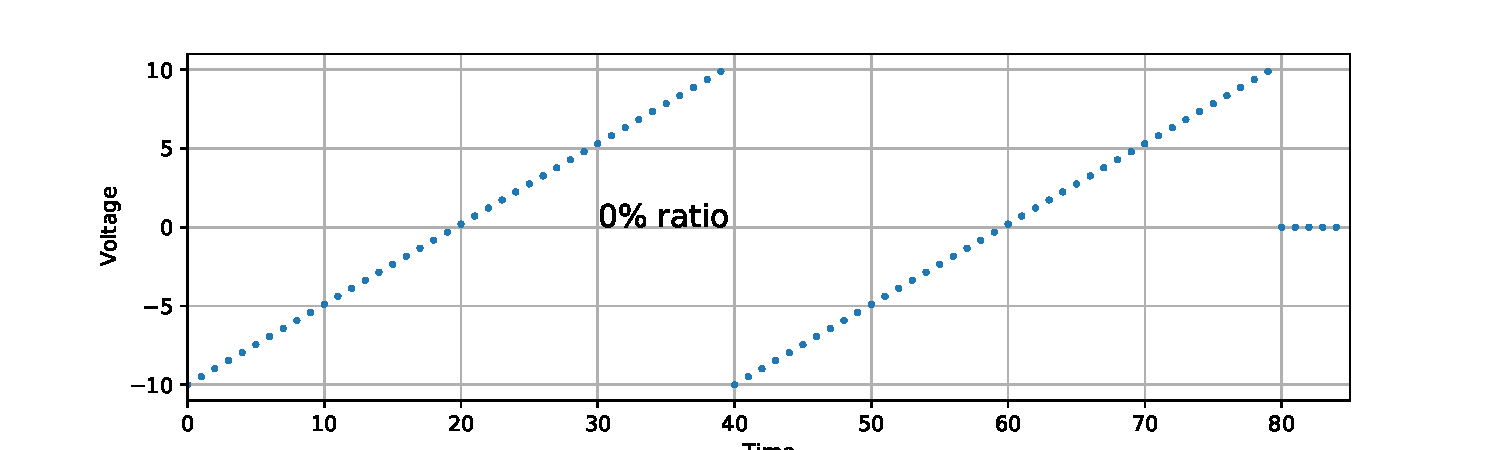
\includegraphics[width=0.95\textwidth]{src/_rampAssymetry0perc.pdf}
		\end{center}
		\begin{center}
		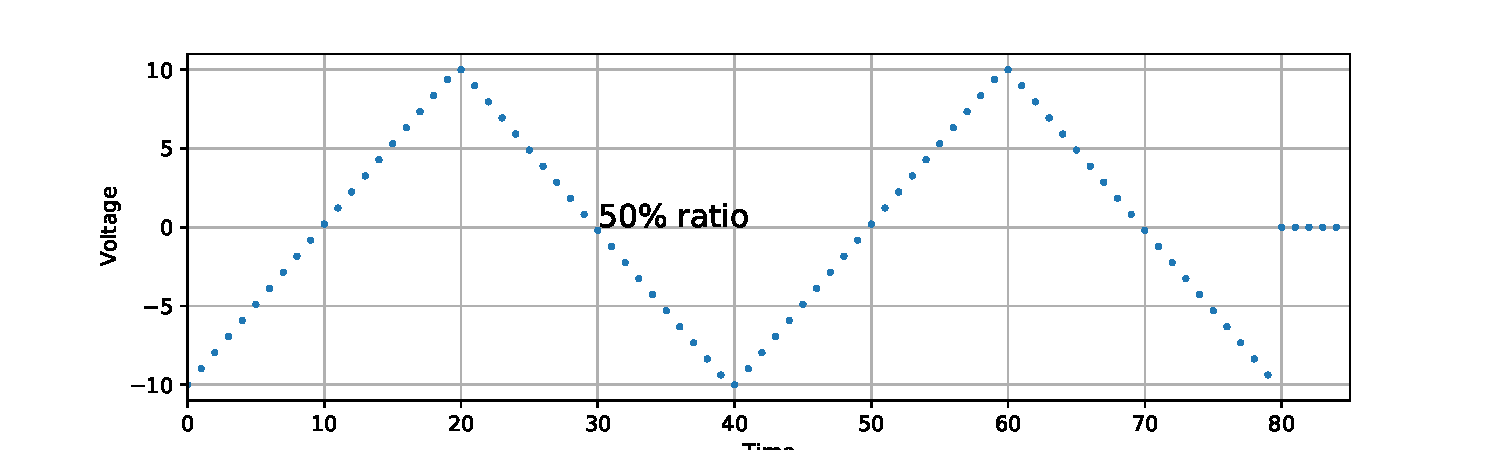
\includegraphics[width=0.95\textwidth]{src/_rampAssymetry50perc.pdf}
		\end{center}
		\begin{center}
		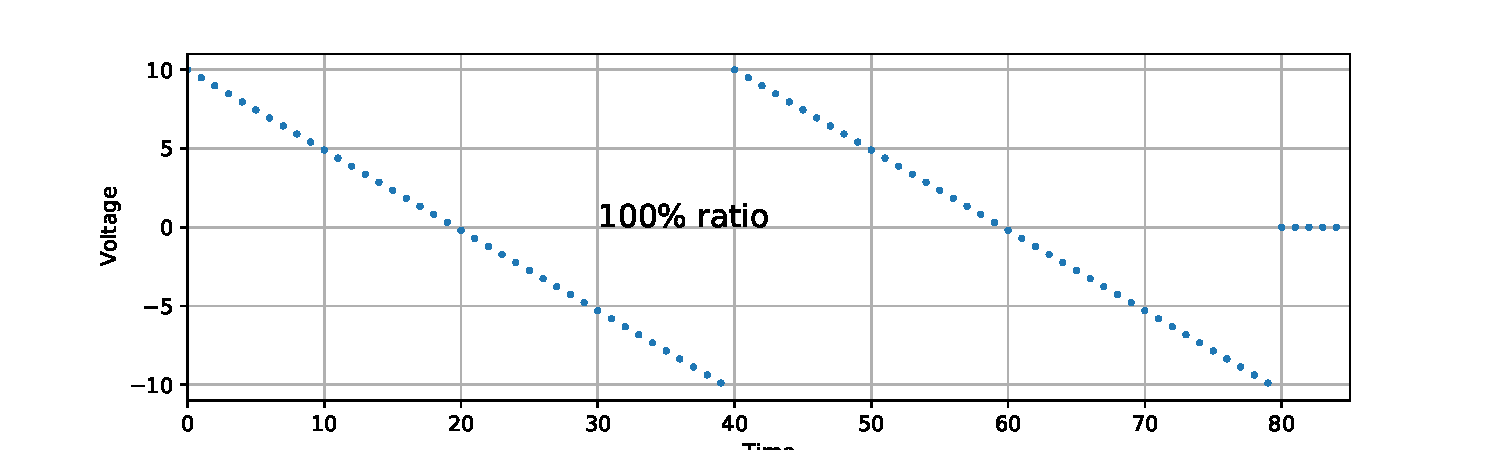
\includegraphics[width=0.95\textwidth]{src/_rampAssymetry100perc.pdf}
		\end{center}


	\req{ RU-21  }{Trigger-IO}{}{}
	{ Internal Trigger-Pulses must be put out via corresponding Trigger-outputs }
	{}{}{}{Triggers}
	\req{ RU-22  }{Trigger-Source}{}{}
	{ Trigger-Modules must be implemented to handle timing of the signal-generation, comprising following input-sources:  $USB$, $Trigger-Input$, $Superior$-$Trigger$, $Push-button$ }
	{}{}{}{Triggers}
	\req{ RU-23  }{Timing-Parameters}{}{}
	{ The FirmWare has to accept signal frequency or signal period and signal vector length as parameters. It has to reply with the actual frequency/period or an error message.}
	{}{}{}{Triggers}
	\req{ RU-24  }{Timing-Calc}{}{}
	{ The FirmWare has to derive necessary sample-rates and trigger-periods from signal period and vector length, either by calculation or by selection from a look-up-table.}
	{}{}{}{Triggers}
	\req{ RU-25  }{Sequences}{}{}
	{ The FirmWare has to generate sequences of A, B and C-Triggers. A-Trigger pulses have a duty-cycle of 50\%, B and C-Trigger have falling edges upon completion.}
	{}{}{}{Triggers}
		\begin{center}
		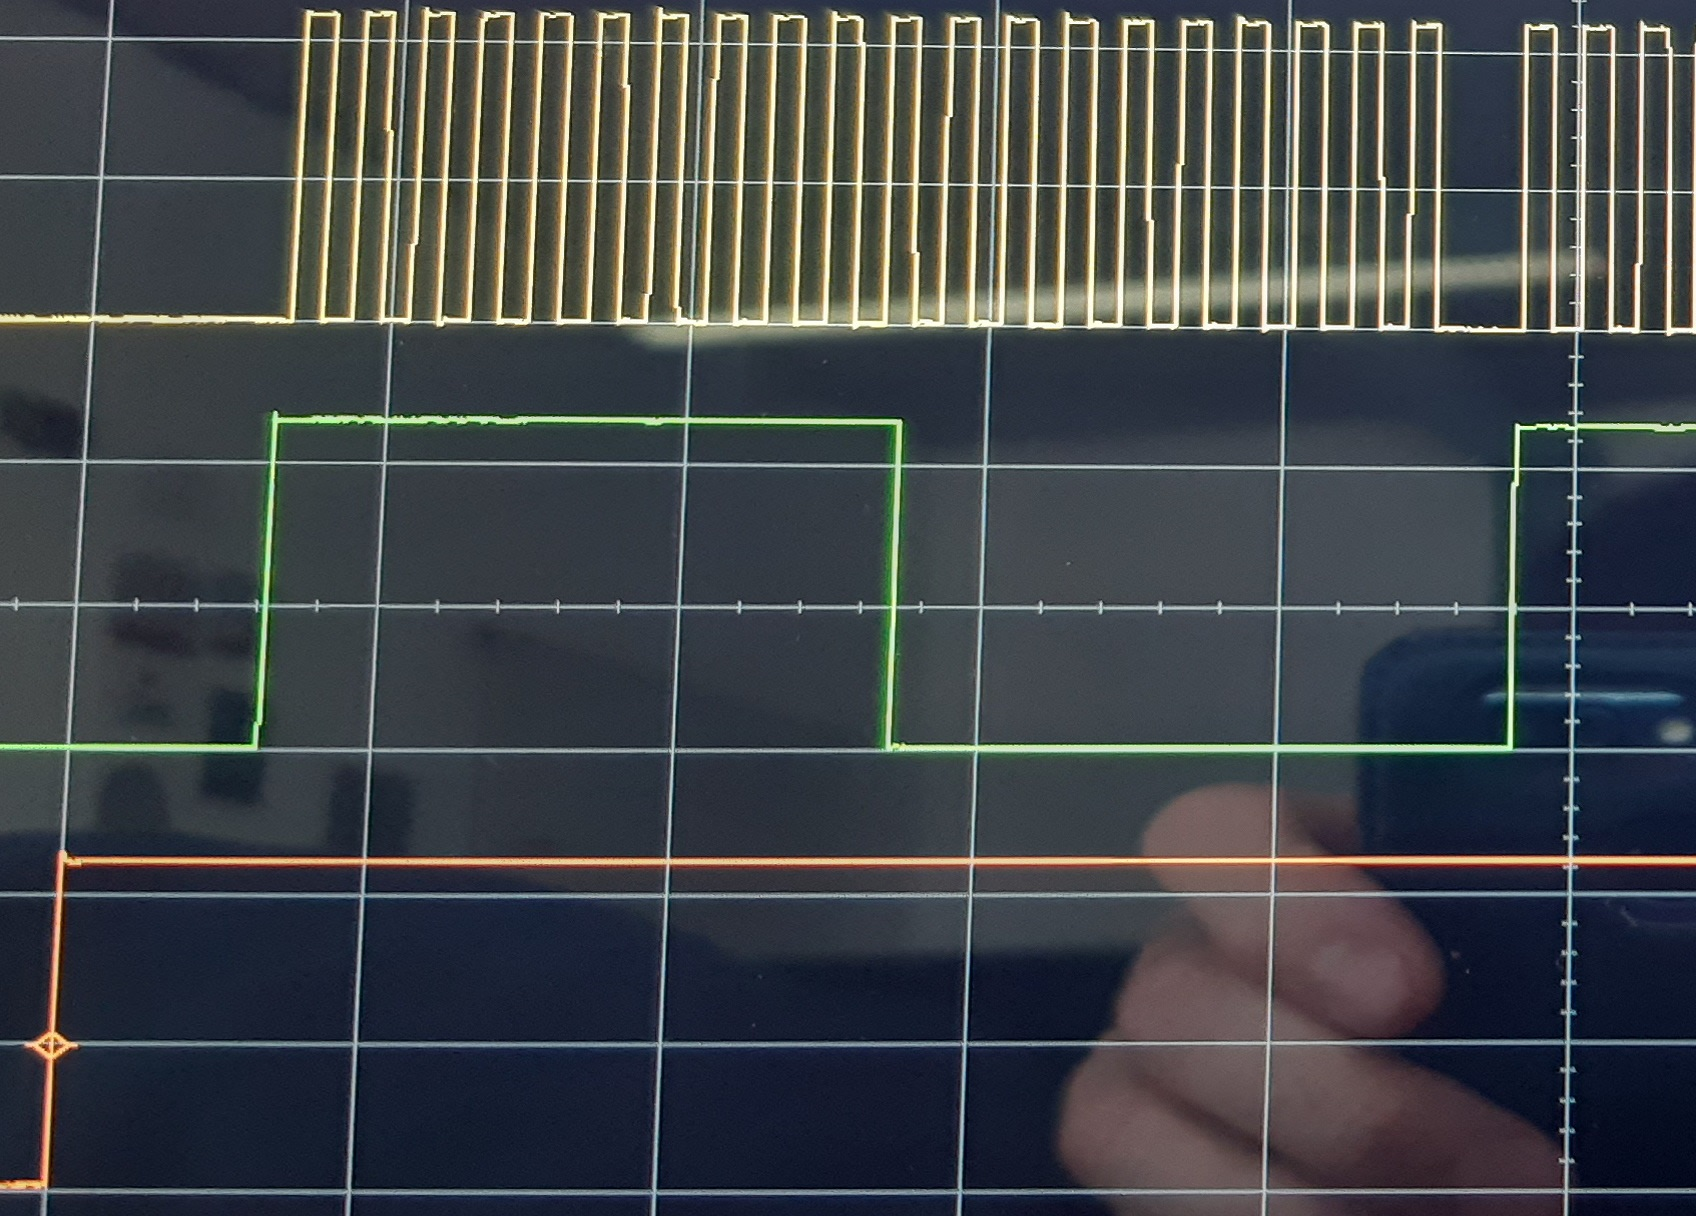
\includegraphics[height=0.2\textheight]{src/_TrigSequence.jpg}
		\end{center}


	\req{ RU-26  }{Buttons,LEDs}{}{}
	{ The FirmWare must access the available push-buttons and state-LEDs. }
	{}{}{}{Miscellaneous}
	\req{ RU-27  }{Button-Function}{}{}
	{ Push-buttons must be programmed to cause transitions to the devices internal state, in a debounced manner. }
	{}{}{}{Miscellaneous}
	\req{ RU-28  }{LED-Function}{}{}
	{ State-LEDs have to represent the current internal state of the device: $idle$, $armed$, $running$ or $error$. }
	{}{}{}{Miscellaneous}
	\req{ RU-29 }{Relays}{}{}
	{ The FirmWare has to provide access to the available relays. Access must consist of $close$, $open$ and $read$-functions }
	{}{}{}{Miscellaneous}
	\req{ RU-30 }{Additional IOs}{}{}
	{ The FirmWare has to provide access for available UART-, $I^2C$-, SPI-modules, as well as digital IOs and analogue inputs.}
	{}{}{}{Miscellaneous}
	\req{ RU-31 }{Additional IO-Modes}{}{}
	{ Functionality for USART-, $I^2C$-, SPI-modules, the digital IOs and analogue inputs must consist of $activation$, $de-activation$, $write$ and $read$.}
	{}{}{}{Miscellaneous}
	\req{ RU-32 }{IO Read}{}{}
	{ $read$-Function must send received information to the host via USB.
	  $read$-Function must be performed upon USB-command, or slave-action.}
	{}{}{}{Miscellaneous}
	\req{ RU-33  }{CRC}{}{}
	{ The FirmWare has to implement functions to perform cyclic-redundancy-check calculations and apply it on verification of incoming strings and adaption of outgoing strings}
	{}{}{}	{Miscellaneous}
	\req{ RU-34  }{Watchdog Functionality \label{WDG}}{ M }{ todo }
	{  The FirmWare has to implement functions to enable the processors built-in watchdog and set its parameters. Available modes have to be $reset$, $powerdown$, $keepalive$}
	{}{}{}	{Miscellaneous}


